\documentclass[t]{beamer}
\usetheme{amcg}
\usepackage{hyperref}
\usepackage{listings}
\setbeamertemplate{navigation symbols}{}

\author[]{Applied Modelling and Computation Group}

\institute{Department of Earth Science and Engineering, Imperial College London}

\date{5-9 November 2012}
\title[Fluidity training - Tides in the Med]{Setting up tides in the Mediterranean.}
\subtitle[]{Fluidity training event}

\setbeamersize{text margin left=0.3in}
\setbeamersize{text margin right=0.3in}

\begin{document}
\titlepage

\begin{frame}{Tutorial overview}
\begin{columns}[l]

\column{3.5in}
The following aspects will be outlined:
  \begin{itemize}
     \item Meshing 
        \begin{itemize}
        \item[$\circ$] Gmsh is used to produce a mesh on a spherical manifold
        \item[$\circ$] An extrusion, creating a 3-D mesh is carried out within fluidity,
              controlled by options in Diamond.
     \end{itemize}
     \item Additional options in Diamond for:
     \begin{itemize}
        \item[$\circ$] Gravity force.
        \item[$\circ$] Coriolis pseudo-force.
        \item[$\circ$] Bottom drag.
        \item[$\circ$] Free surface.
        \item[$\circ$] Tidal forcing.
     \end{itemize}

  \end{itemize}

Example available in directory:\\
{\it trunk/examples/tides\_in\_the\_Mediterranean\_Sea}

\column{1.5in}
\vspace{-0.9in}
\begin{figure}[htbp!]
 \centering
  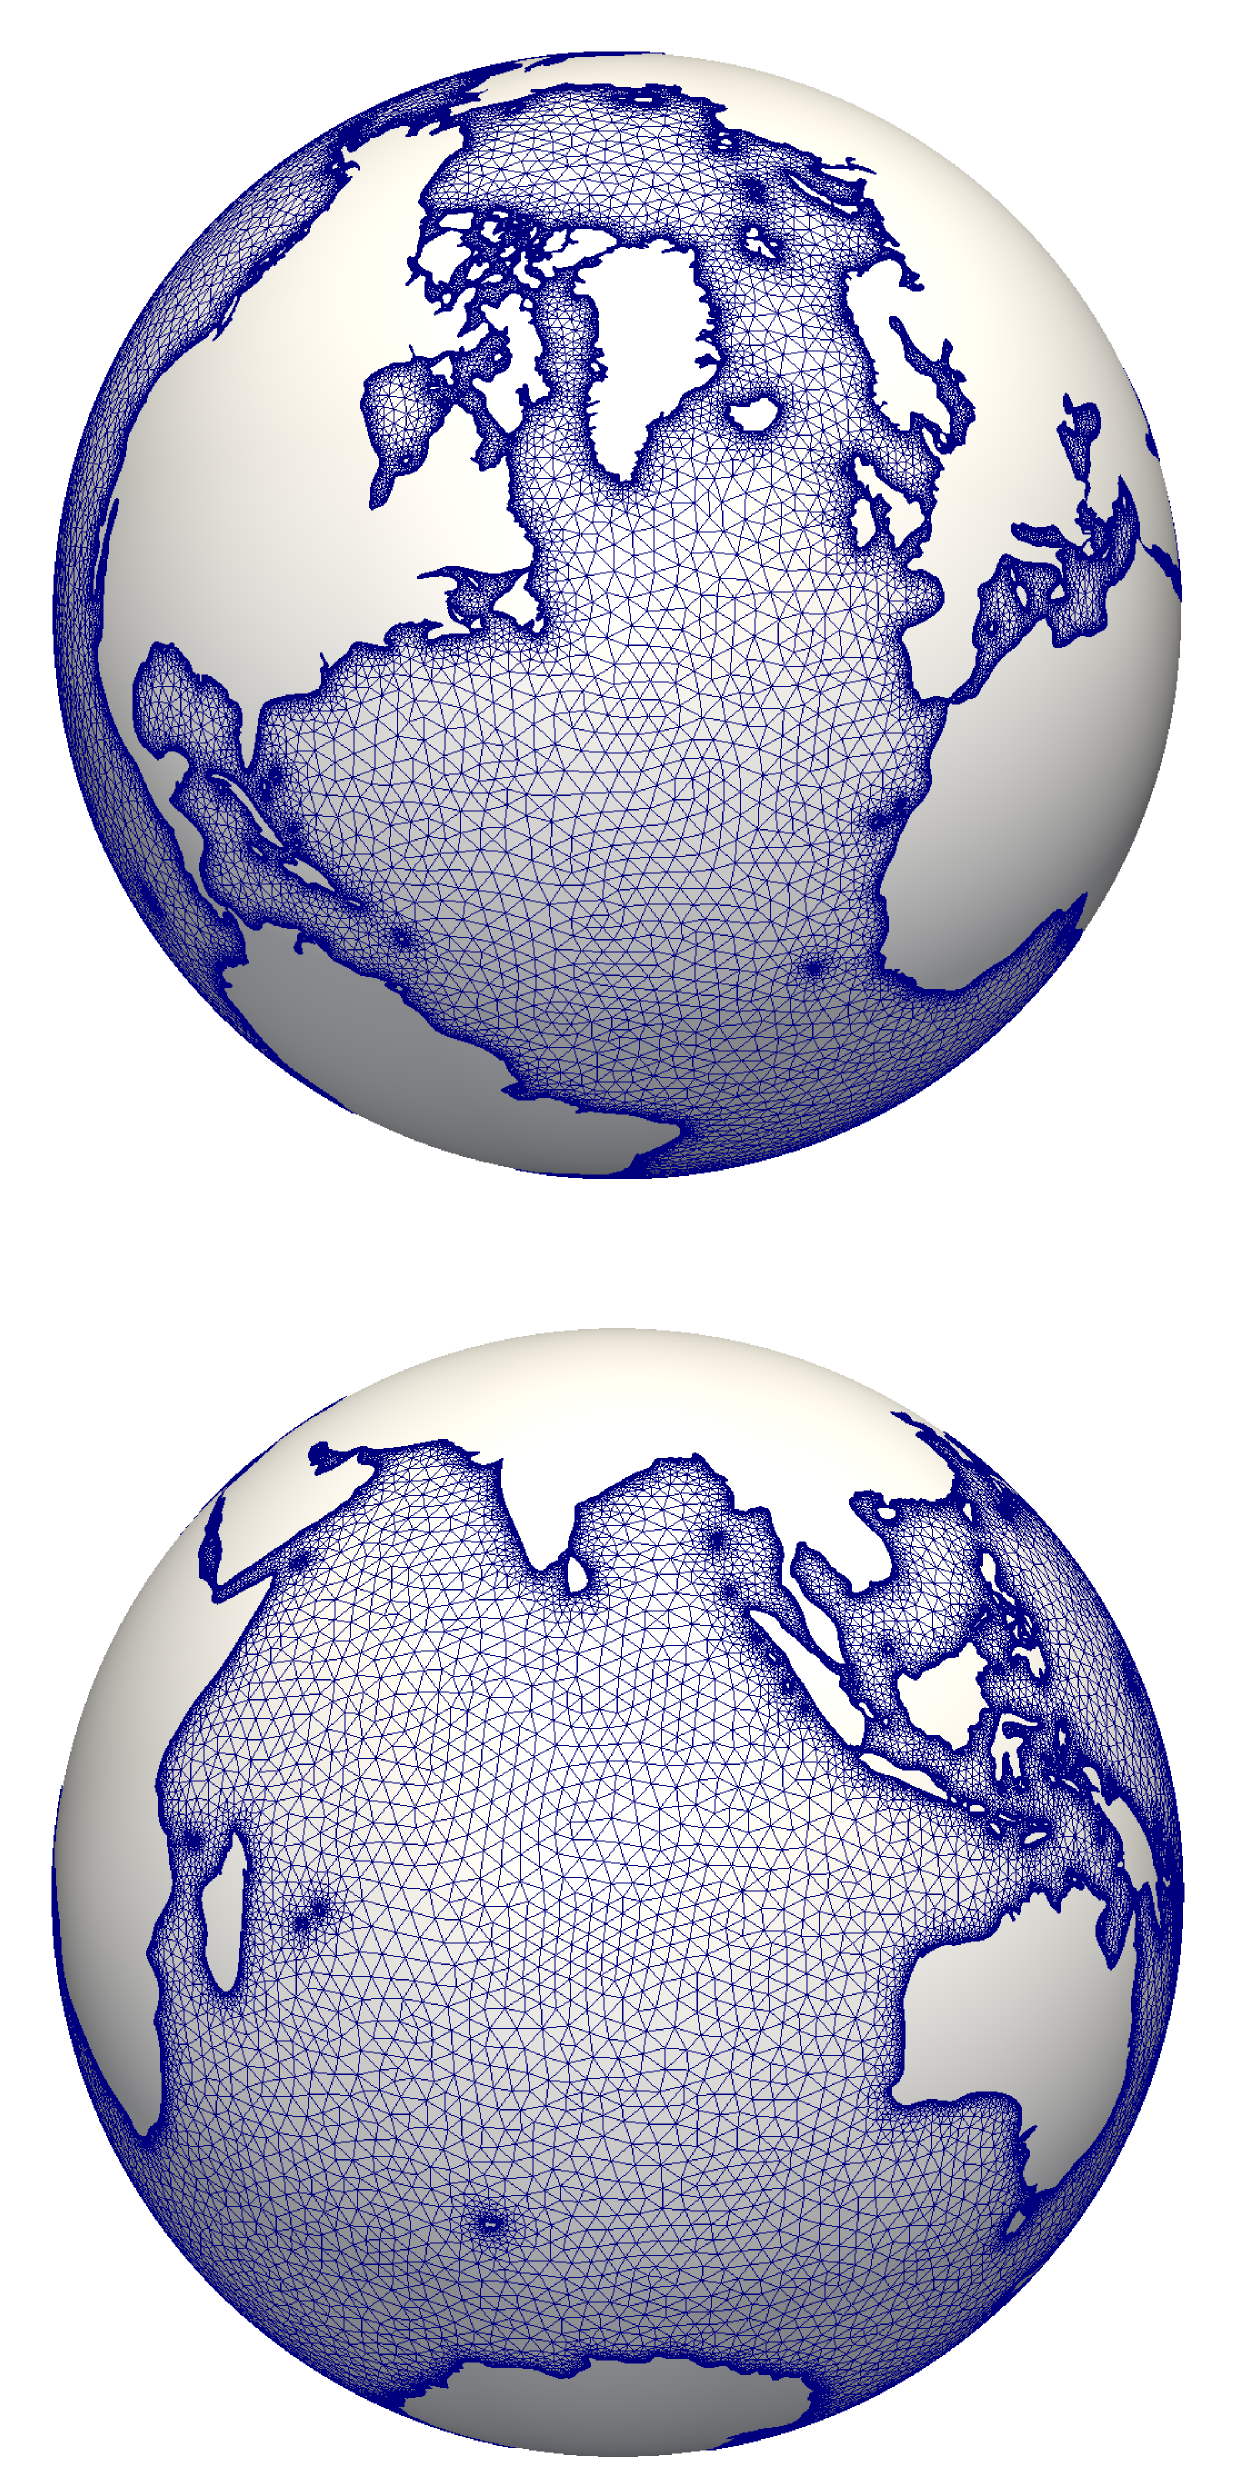
\includegraphics[width=1.0\textwidth]{figures/globe_mesh}
\end{figure}

\end{columns}

\end{frame}

\begin{frame}{2-D mesh in Gmsh}

\begin{figure}[htbp!]
 \centering
  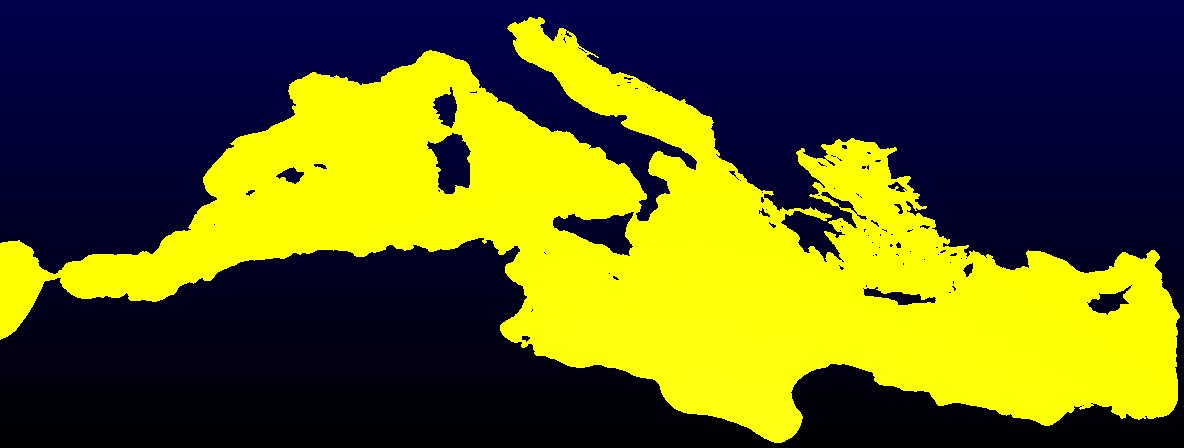
\includegraphics[width=0.6\textwidth]{figures/med_mesh2}
\end{figure}
\begin{itemize}
\item Mesh is generated on a spherical shell.
\\ Tutorial {\footnotesize \url{http://amcg.ese.ic.ac.uk/files/gmsh\_tutorial.pdf}} or \\ {\footnotesize \url{http://perso.uclouvain.be/jonathan.lambrechts/gmsh_ocean/}}
\item Coastlines extracted from GSHHS dataset.
\item Mesh available in {\it trunk/examples/tides\_in\_the\_Mediterranean\_Sea/med.msh}
\end{itemize}

\end{frame}

\begin{frame}{Extruding in Fluidity}
\begin{itemize}
\item 2-D horizontal mesh is extruded vertically within Fluidity.
\end{itemize}
\begin{figure}[htbp!]
 \centering
  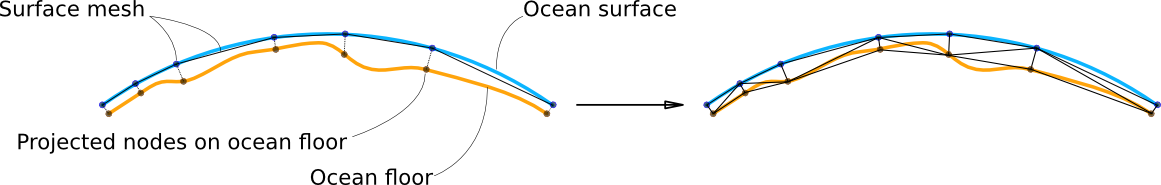
\includegraphics[width=1.0\textwidth]{figures/mesh_extrusion.png}
\end{figure}
\begin{itemize}
\item Flexibility to choose layered $\sigma$ or $z$-coordinates.
\item Bathymetry extracted from NetCDF file ({\it e.g.} $GEBCO$ dataset.)
\end{itemize}

\begin{figure}[htbp!]
 \centering
  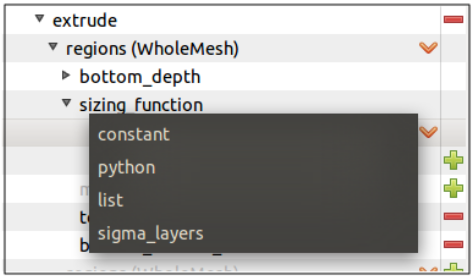
\includegraphics[width=0.3\textwidth]{figures/extrude}
\end{figure}

\end{frame}

\begin{frame}{Extruding: Spherical Earth's surface representation}
\begin{itemize}
  \item Linear mapping
  \begin{itemize}
    \item[$\circ$] Element faces on sea surface are flat.
    \item[$\circ$] Appropriate choice for P1 grids.
    \item[$\circ$] Suitable for barotropic simulations.
  \end{itemize}
  \item Super-parametric mapping
  \begin{itemize}
    \item[$\circ$] Element faces on sea surface are described by $n^{th}$ order polynomials
    \item[$\circ$] Order of polynomial equal to the degree of the mesh.
    \item[$\circ$] Suitable for baroclinic simulations (currently up to 2nd order in parallel).
  \end{itemize}
\end{itemize}

\end{frame}

\begin{frame}{Gravity, Coriolis \& Bottom drag}
\begin{itemize}
  \item Gravity force and Coriolis pseudo-force are set under physical parameters
  \begin{itemize}
    \item[$\circ$] Gravity magnitude and direction
    \item[$\circ$] Coriolis ($f$-, $\beta$-plane, on-sphere)
  \end{itemize}
  \item Ocean floor: no-normal-flow \& drag wall-law,
  \begin{align*}
  \frac{\partial u}{\partial z} \propto D_{bottom} = \frac{1}{2} C_D \rho u^{2}
  \end{align*}
  set as boundary condition on velocity:
\end{itemize}
\begin{figure}[htbp!]
 \centering
  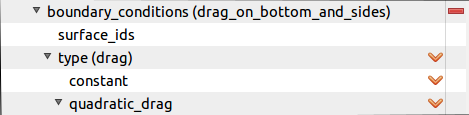
\includegraphics[width=0.6\textwidth]{figures/bottom_drag}
\end{figure}
\end{frame}

\begin{frame}{Setting the free surface}
\begin{itemize}
  \item Free surface: Kinematic boundary condition on velocity.
  \begin{itemize}
    \item[$\circ$] The velocity of a particle at the surface is tangential to the surface.
  \end{itemize}
\end{itemize}

\begin{columns}[l]
\column{2.5in}
  \begin{align*}
    -\overrightarrow{n}_s \cdot \overrightarrow{n}_g\frac{\partial h}{\partial t} = \overrightarrow{n}_s \cdot \overrightarrow{u}
  \end{align*}

\column{2.5in}
  \begin{figure}[htbp!]
   \centering
    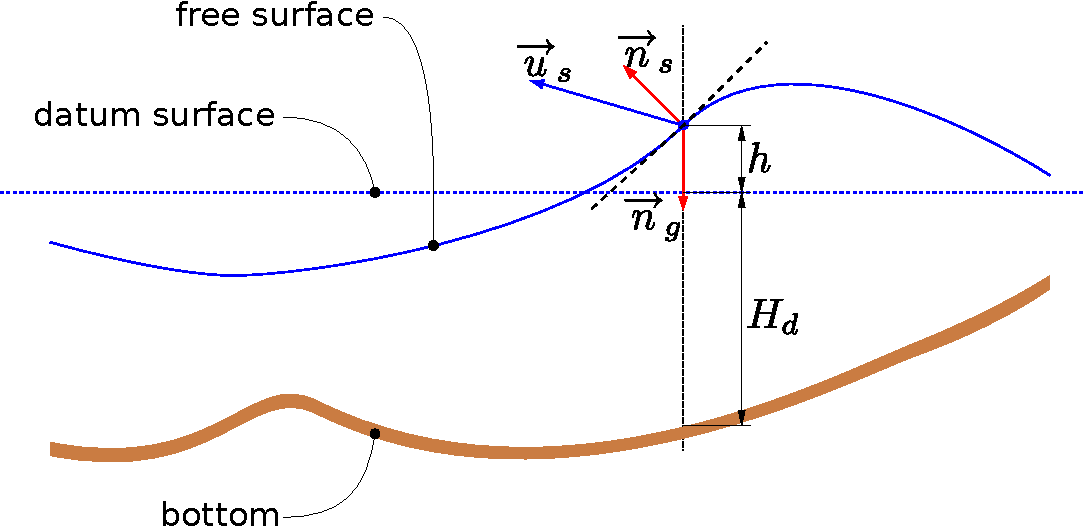
\includegraphics[width=0.8\textwidth]{figures/free_surface}
  \end{figure}
\end{columns}

\begin{figure}[htbp!]
 \centering
  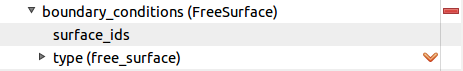
\includegraphics[width=0.6\textwidth]{figures/freesurface}
\end{figure}

\end{frame}

\begin{frame}{Setting the tidal forcing-body forcing}
  \begin{itemize}
  \item Astronomical body forcing.
    \begin{itemize}
       \item[$\circ$] Specify the tidal components.
    \end{itemize}
  \end{itemize}
  \begin{figure}[htbp!]
    \centering
    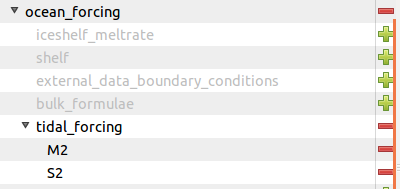
\includegraphics[width=0.7\textwidth]{figures/body_forcing}
  \end{figure}
\end{frame}

\begin{frame}{Setting the tidal forcing-free surface elevation at boundary}
  \begin{itemize}
  \item Dirichlet boundary condition on pressure at open boundaries.
    \begin{itemize}
       \item[$\circ$] Pressure set for free-surface elevation to match observational data
    \end{itemize}
  \item User has to specify:
    \begin{itemize}
       \item[$\circ$] Which tidal components.
       \item[$\circ$] NetCDF file to read free-surface elevation from.
       \item[$\circ$] Name of phase \& magnitude variables in file.
    \end{itemize}
  \end{itemize}
  \begin{figure}[htbp!]
    \centering
    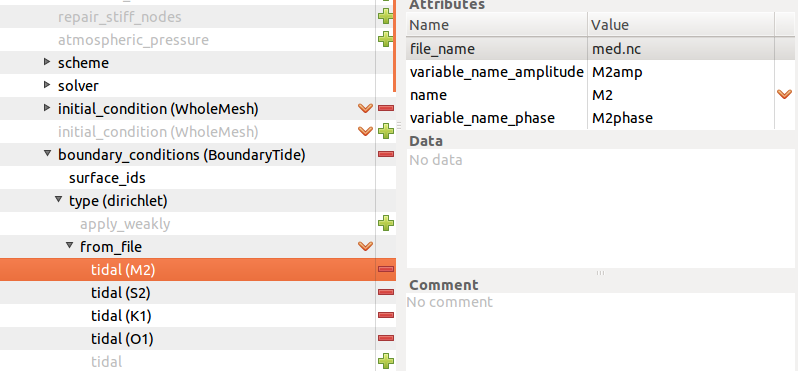
\includegraphics[width=0.6\textwidth]{figures/diamond_freeSurf_pre_Bc.png}
  \end{figure}
\end{frame}

\end{document}
